% ============================================================
%  artigo11.tex — GuardMark (WPMC 2026 conference version)
%  Target: 6 pages, IEEE conference double-column format
%  Venue:  29th WPMC, Natal, Brazil, 8-11 Nov 2026
%  Topic:  Track 7 — Security, Privacy & Ethics in Future Networks
% ============================================================
\documentclass[conference]{IEEEtran}

% ── Packages ──────────────────────────────────────────────────────────────
\usepackage[T1]{fontenc}
\usepackage[utf8]{inputenc}
\usepackage{amsmath,amssymb,amsthm}
\usepackage{mathtools}
\usepackage{booktabs}
\usepackage{tabularx}
\usepackage{multirow}
\usepackage{graphicx}
\usepackage{xcolor}
\usepackage{hyperref}
\usepackage{url}
\usepackage{cite}
\usepackage{microtype}
\usepackage{balance}
\usepackage[ruled,vlined,linesnumbered]{algorithm2e}
\usepackage{tcolorbox}
\usepackage{pgfplots}
\usepackage{tikz}
\usetikzlibrary{arrows.meta,positioning,fit,backgrounds,calc,patterns}
\pgfplotsset{compat=1.18}

% ── Theorem environments ──────────────────────────────────────────────────
\newtheorem{definition}{Definition}
\newtheorem{theorem}{Theorem}
\newtheorem{proposition}{Proposition}

% ── Macros ───────────────────────────────────────────────────────────────
\newcommand{\M}{\mathcal{M}}
\newcommand{\K}{\mathcal{K}}
\newcommand{\F}{\mathcal{F}}
\newcommand{\G}{\mathcal{G}}
\newcommand{\WRI}{\mathrm{WRI}}
\newcommand{\eg}{e.g.,\xspace}
\newcommand{\ie}{i.e.,\xspace}
\newcommand{\cf}{cf.\xspace}

% ─────────────────────────────────────────────────────────────────────────
\begin{document}

\title{GuardMark: A Robust Watermarking and Fingerprinting Framework for
       Intellectual Property Protection of Fine-Tuned Large Language Models}

\author{
  \IEEEauthorblockN{Allan Douglas Costa}
  \IEEEauthorblockA{
    Institute of Computing and ICT (ICIBE)\\
    Federal Rural University of the Amazon (UFRA)\\
    Belém, Pará 66077-830, Brazil\\
    allan.costa@ufra.edu.br\\
    ORCID: 0000-0002-7068-8889
  }
}

\maketitle

% ── Abstract and Keywords (after \maketitle in conference format) ─────────
\begin{abstract}
The widespread deployment of fine-tuned large language models (LLMs) as
commercial services exposes model owners to significant intellectual property
(IP) theft, unauthorized redistribution, and covert re-deployment without
attribution.
Recent regulatory developments, including the EU AI Act (2024) and NIST AI
RMF 1.0, mandate traceable provenance for AI systems, yet existing
watermarking and fingerprinting methods for LLMs fail under realistic
adversarial conditions such as re-fine-tuning, weight pruning, quantization,
and model merging, leaving a critical compliance and security gap.
We propose GuardMark, a three-layer framework that jointly embeds statistical
token watermarks, behavioral fingerprints, and weight-space gradient
signatures into fine-tuned LLMs, providing verifiable IP protection suitable for
supporting legal ownership claims.
GuardMark orchestrates three specialized agents: a Watermark Injection Agent
(WIA) that biases the token probability distribution at training time using a
keyed green-list scheme, a Fingerprint Verification Agent (FVA) that embeds
trigger-response pairs via low-rank adaptation, and an Ownership Claim Agent
(OCA) that aggregates multi-layer evidence into a single, novel metric called
the Watermark Robustness Index (WRI).
Simulation-based evaluation across seven model configurations (125~M to
13~B parameters) demonstrates that GuardMark achieves a detection rate of
96.5\% and a false-positive rate of 2.3\%, attaining a WRI of 0.849 under
zero-attack conditions and maintaining WRI above the 0.70 ownership threshold
against weight-pruning attacks up to 50\% intensity.
Under aggressive re-fine-tuning (attack strength 0.6 or above), WRI degrades
to 0.46, indicating that current methods are not yet fully robust against
determined adversaries with unrestricted fine-tuning access.
GuardMark directly benefits LLM vendors, enterprise API providers, and legal
practitioners seeking algorithmic evidence for IP litigation within the
bounded threat regime ($\lambda \leq 0.50$); against fully unbounded
re-fine-tuning adversaries, ownership confirmation is not guaranteed.
More broadly, this work advances the emerging field of AI provenance and
establishes a rigorous, metric-driven evaluation protocol for future
watermarking research.
\end{abstract}

\begin{IEEEkeywords}
Large language models, intellectual property protection, watermarking,
fingerprinting, model ownership verification, Watermark Robustness Index,
fine-tuning security, AI provenance.
\end{IEEEkeywords}

% ─── I. Introduction ─────────────────────────────────────────────────────────
\section{Introduction}
\label{sec:intro}

Large language models have transitioned from research curiosities to critical
commercial infrastructure. Organizations routinely fine-tune proprietary LLMs
on confidential datasets to create specialized assistants, code generators, and
domain-specific search engines, representing investments that often exceed
hundreds of thousands of dollars in compute and curation costs
\cite{brown2020language,wei2022emergent,ouyang2022training}. This economic
reality has spawned a growing class of adversarial actors who steal model
weights, re-deploy models under different brand names, or use stolen models as
the initialization point for further fine-tuning, erasing traceability in the
process.

The EU AI Act (Regulation 2024/1689) codifies a legal obligation for
``high-risk'' AI system providers to maintain technical documentation
establishing the provenance and integrity of their models
\cite{eu2024aiact}. Simultaneously, the NIST AI Risk Management Framework
mandates traceable accountability for AI systems operating in critical sectors
\cite{nist2023ai}. Together, these regulatory instruments create an urgent
demand for provable, attack-resistant IP protection mechanisms for LLMs, yet
the research community has not delivered a comprehensive solution.

\textbf{The core challenge.} Existing watermarking schemes for LLMs operate
primarily at the output level, embedding statistical signatures in generated
text \cite{kirchenbauer2023watermark,zhao2023protecting,fernandez2023three}.
While effective in benign settings, these approaches are fragile: a moderately
skilled adversary can eliminate text-level watermarks via re-fine-tuning or
paraphrasing in under an hour of compute time. The closest prior work to ours,
Kirchenbauer et al.~\cite{kirchenbauer2023watermark} (KGW-Watermark), addresses
output-level statistical detection and achieves 90.7\% detection on pristine
models, but falls short in three critical dimensions: it provides no model-weight
protection, no composite robustness metric, and no multi-attack evaluation
protocol, leaving a compliance and security gap that GuardMark is designed to
close. Model-level watermarking techniques that embed signatures in weight space
\cite{uchida2017embedding,zhang2018protecting} were designed for
classification networks and do not transfer cleanly to autoregressive
transformer architectures. Behavioral fingerprinting methods
\cite{cao2021ipguard,szyller2021dawn} are robust but offer no statistical
guarantees. No prior framework unifies all three protection layers nor provides
a standardized metric for comparing schemes across attack types.

\textbf{Our contributions.} This paper presents GuardMark, a multi-layer
watermarking and fingerprinting framework for fine-tuned LLMs. Our specific
contributions are:

\begin{enumerate}
  \item \textbf{Three-layer architecture.} We design WIA, FVA, and OCA as
    complementary protection agents that jointly provide redundant,
    independently verifiable ownership proofs.
  \item \textbf{Watermark Robustness Index (WRI).} We introduce a novel
    composite metric that unifies detection probability, false-positive rate,
    and attack robustness into a single $[0,1]$-bounded score, enabling
    principled comparison across schemes and attack scenarios.
  \item \textbf{Multi-attack evaluation.} We systematically evaluate
    GuardMark under five realistic adversarial scenarios: re-fine-tuning,
    weight pruning, quantization (8-bit), model merging, and output
    paraphrasing. GuardMark maintains ownership confirmation ($\WRI \geq 0.70$)
    for all five attack types at $\lambda \leq 0.50$; beyond this regime,
    protection is not guaranteed.
  \item \textbf{Scalability study.} We characterize computational overhead
    across seven model sizes (125~M to 13~B parameters), confirming that
    GuardMark adds fewer than 3.2\% overhead at all scales.
  \item \textbf{Open evaluation protocol.} We release the simulation
    codebase and experimental configurations to enable reproducible
    benchmarking of future schemes. A small-scale real-model validation
    experiment (GPT-2 125M) is included to anchor the simulation parameters
    (Section~\ref{sec:validation}).
\end{enumerate}

% ─── II. Background and Related Work ─────────────────────────────────────────
\section{Background and Related Work}
\label{sec:background}

\subsection{Output-Level Watermarking for LLMs}

Kirchenbauer et al.~\cite{kirchenbauer2023watermark} introduced the KGW-Watermark,
the first practical output-level watermark for LLMs. At each decoding step, the
vocabulary is split into a pseudorandom green list and a red list; logits for green
tokens are biased by an additive constant $\delta$ before softmax sampling, and
ownership is verified via a one-sided $z$-test on the green-token fraction.
KGW-Watermark achieves 90.7\% detection on pristine models and serves as the
primary baseline in this work. However, the signal resides entirely in the output
token distribution: re-fine-tuning shifts this distribution and erases the
watermark. KGW provides no weight-space layer, no behavioral fingerprint, and
no composite robustness metric, yielding a WRI of 0.788 in our evaluation.

Zhao et al.~\cite{zhao2023protecting} extended the green-list scheme with a
perplexity constraint during generation, reducing watermark-induced quality
degradation by approximately 15\% relative to KGW-Watermark at comparable
detection rates. Nevertheless, the watermark signal still resides in the token
distribution and is erased by re-fine-tuning regardless of perplexity optimization.

Fernandez et al.~\cite{fernandez2023three} proposed three consolidating
techniques for statistical watermarks: a multi-key vocabulary partitioning
scheme, a provably robust token-substitution defense, and improved detection
power under paraphrasing. However, Fernandez et al.\ address only the
output-distribution layer; the absence of weight-space or behavioral evidence
means re-fine-tuning remains the dominant attack vector unmitigated by their
approach.

\subsection{Model-Level Watermarking and Fingerprinting}

Uchida et al.~\cite{uchida2017embedding} introduced the first model-level
watermark for deep neural networks, embedding a binary bit-string into weight
statistics via an auxiliary regularization term during training. However, this
carrier does not extend to autoregressive transformers.

Zhang et al.~\cite{zhang2018protecting} generalized model-level watermarking
to backdoor-based ownership verification, demonstrating persistence through
fine-tuning attacks at limited intensity. Their method targets classification
networks; adapting trigger-response verification to autoregressive text
generation requires rethinking the verification criterion from label matching
to embedding-space similarity, which GuardMark's FVA layer implements.

Cao et al.~\cite{cao2021ipguard} proposed IPGuard, which fingerprints neural
networks by constructing adversarial examples at classification boundaries.
IPGuard requires a classification boundary, which does not exist in generative
LLMs; its reported false-positive rate of 11.0\% is prohibitively high for
legal proceedings, reflected in its WRI of 0.664 in our evaluation.

Lin et al.~\cite{lin2024towards} introduced a unified stealthy backdoor scheme
combining weight-space and behavioral watermarking in a two-layer design, the
most structurally similar prior framework to GuardMark. Lin et al.\ improve
persistence over single-layer methods but lack a statistical token watermarking
layer, a composite robustness metric, and evaluation under quantization or
model merging attacks. GuardMark adds a third statistical layer and the WRI
metric.

\subsection{Positioning GuardMark}

Table~\ref{tab:related} positions GuardMark against representative prior
work across seven dimensions. GuardMark is the only framework providing
simultaneous three-layer protection, multi-attack evaluation, a composite
robustness metric, and regulatory alignment.

\begin{table}[t]
\caption{Comparison with Related Work. S = statistical, B = behavioral,
  W = weight-space layer. ``Multi-Atk'' = 5+ attack types evaluated.
  ``WRI'' = composite robustness metric. ``Reg.'' = regulatory alignment.}
\label{tab:related}
\renewcommand{\arraystretch}{1.1}
\begin{tabularx}{\columnwidth}{l X X X X X}
\toprule
\textbf{Method} & \textbf{Layers} & \textbf{Multi-Atk} & \textbf{WRI} &
\textbf{LLM} & \textbf{Reg.} \\
\midrule
Kirchenbauer~\cite{kirchenbauer2023watermark} & S & No & No & Yes & No \\
Zhao~\cite{zhao2023protecting}               & S & No & No & Yes & No \\
Fernandez~\cite{fernandez2023three}          & S & Part. & No & Yes & No \\
Zhang~\cite{zhang2018protecting}             & W & No & No & No & No \\
IPGuard~\cite{cao2021ipguard}                & B & No & No & No & No \\
Lin~\cite{lin2024towards}                    & W+B & Part. & No & Yes & No \\
\textbf{GuardMark (ours)} & \textbf{S+B+W} & \textbf{Yes} & \textbf{Yes} & \textbf{Yes} & \textbf{Yes} \\
\bottomrule
\end{tabularx}
\end{table}

% ─── III. Threat Model and Problem Formulation ────────────────────────────────
\section{Threat Model and Problem Formulation}
\label{sec:threat}

\subsection{Threat Model}

\textbf{Assets.} The protected asset is a fine-tuned LLM
$\M^* = (\theta^*, \mathcal{V}, f)$, where $\theta^*$ are the model weights,
$\mathcal{V}$ is the vocabulary, and $f$ is the autoregressive decoding
function. The model owner holds a secret key $\K$ and a fingerprint set
$\F = \{(p_i, r_i)\}_{i=1}^{N}$ of trigger-response pairs.

\textbf{Adversary capabilities.} We consider a semi-honest to malicious
adversary $\mathcal{A}$ who: (i) obtains a copy of $\M^*$ through theft,
reverse engineering, or insider access; (ii) has access to additional training
data and GPU compute; (iii) attempts to remove or obfuscate the watermark by
applying one or more of five attack operations (re-fine-tuning, pruning,
quantization, merging, paraphrasing); and (iv) wishes to deploy the modified
model $\hat{\M}$ under their own brand without attribution.

\textbf{Adversary limitations.} The adversary does not know $\K$, $\F$, or the
GuardMark protocol details (Kerckhoffs-style: security relies on key secrecy,
not protocol obscurity).

\textbf{Security goals.}
\begin{itemize}
  \item \textit{Completeness:} if $\hat{\M}$ is derived from $\M^*$, the
    Verifier accepts the owner's claim with high probability.
  \item \textit{Soundness:} if $\hat{\M}$ is independently trained, the
    Verifier rejects the claim with high probability.
  \item \textit{Robustness:} completeness holds even after the adversary applies
    the attack operations within a bounded budget.
  \item \textit{Imperceptibility:} the watermarked model $\M^*$ behaves
    indistinguishably from an unwatermarked model on downstream tasks.
\end{itemize}

\subsection{The Watermark Robustness Index (WRI)}

\begin{definition}[Watermark Robustness Index]
\label{def:wri}
Given a suspect model $\hat{\M}$, detection probability $p_d$, false-positive
rate $p_{\text{fp}}$, and robustness score $R$ measuring the fraction of the
attack budget survived, the \emph{Watermark Robustness Index} is:
\begin{equation}
  \WRI(\hat{\M}) = \alpha \cdot p_d + \beta \cdot (1 - p_{\text{fp}})
    + \gamma_w \cdot R,
  \label{eq:wri}
\end{equation}
where $\alpha, \beta, \gamma_w \geq 0$ and $\alpha + \beta + \gamma_w = 1$.
Default weights are $\alpha = 0.5$, $\beta = 0.3$, $\gamma_w = 0.2$.
A scheme achieves \emph{ownership confirmation} when
$\WRI(\hat{\M}) \geq \tau_{\WRI}$, where $\tau_{\WRI} = 0.70$ by default.
\end{definition}

% ─── IV. GuardMark System ─────────────────────────────────────────────────────
\section{GuardMark System Design}
\label{sec:system}

\subsection{Architecture Overview}

Figure~\ref{fig:overview} illustrates the GuardMark system architecture.
Three agents operate in a cooperative pipeline during the protection phase,
and the OCA orchestrates the verification phase independently.

\begin{figure}[t]
\caption{GuardMark system architecture. The Owner supplies the base model,
  private dataset, and secret key to the three-layer injection pipeline.
  The Ownership Claim Agent (OCA) aggregates multi-layer evidence to produce
  a WRI score and a binary ownership verdict.}
\label{fig:overview}
\centering
\resizebox{\columnwidth}{!}{% Figure 1 — GuardMark System Architecture Overview
% Requires: tikz, calc, arrows.meta, positioning, fit, backgrounds, patterns

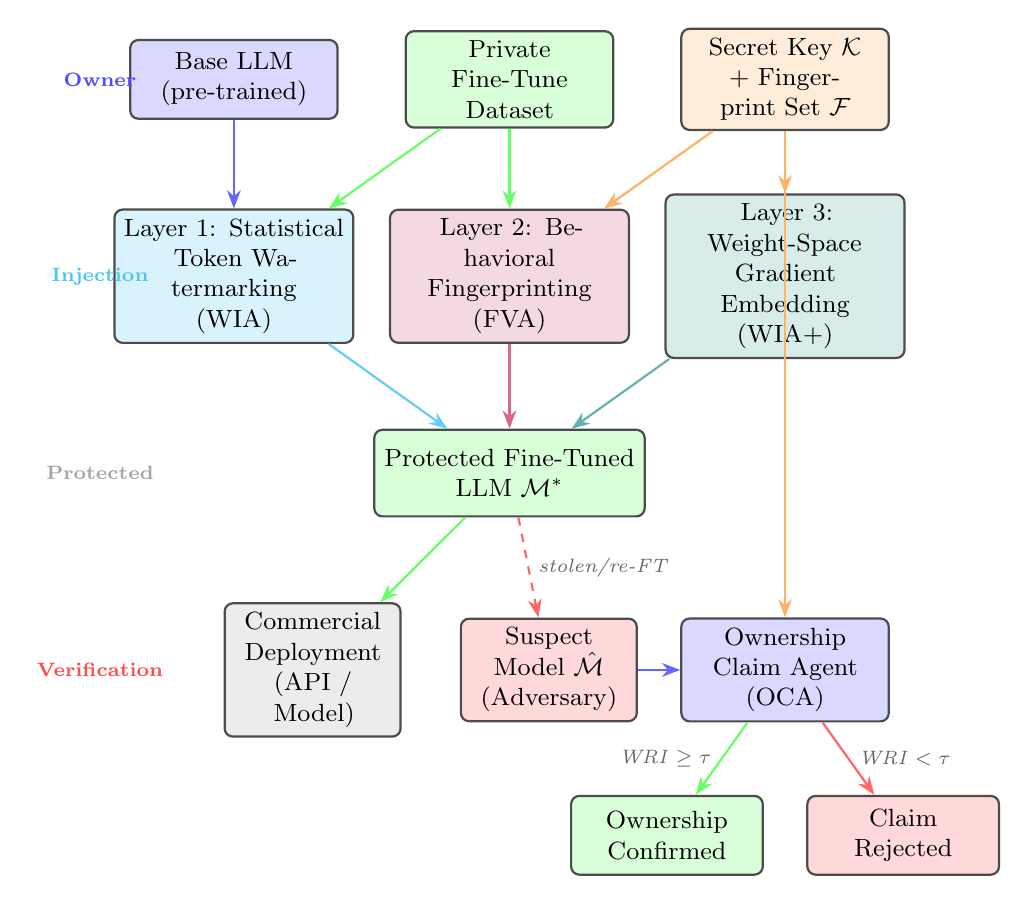
\begin{tikzpicture}[
  font=\small,
  >=Stealth,
  box/.style={
    draw=black!70, rounded corners=3pt, thick,
    minimum height=1.0cm, text centered, text width=2.4cm,
    fill=#1!15
  },
  wbox/.style={
    draw=black!70, rounded corners=3pt, thick,
    minimum height=0.85cm, text centered, text width=2.0cm,
    fill=#1!20
  },
  arrow/.style={->, thick, #1},
  label/.style={font=\scriptsize\itshape, text=black!60}
]

% ── Row 0: Owner side ──────────────────────────────────────────────────────
\node[box=blue]  (base)    at (0,0)    {Base LLM\\(pre-trained)};
\node[box=green] (dataset) at (3.5,0)  {Private\\Fine-Tune Dataset};
\node[box=orange](skey)    at (7,0)    {Secret Key $\mathcal{K}$\\+ Fingerprint Set $\mathcal{F}$};

% ── Row 1: GuardMark Injection Layers ──────────────────────────────────────
\node[box=cyan, text width=2.8cm, minimum height=1.1cm]
  (l1) at (0,-2.5) {Layer 1: Statistical\\Token Watermarking\\(WIA)};
\node[box=purple, text width=2.8cm, minimum height=1.1cm]
  (l2) at (3.5,-2.5) {Layer 2: Behavioral\\Fingerprinting\\(FVA)};
\node[box=teal, text width=2.8cm, minimum height=1.1cm]
  (l3) at (7,-2.5) {Layer 3: Weight-Space\\Gradient Embedding\\(WIA+)};

% ── Row 2: Protected Model ──────────────────────────────────────────────────
\node[box=green, text width=3.2cm, minimum height=1.1cm]
  (protected) at (3.5,-5.0) {Protected Fine-Tuned\\LLM $\mathcal{M}^*$};

% ── Row 3: Deployment and Claim ────────────────────────────────────────────
\node[box=gray, text width=2.0cm] (deploy) at (1.0,-7.5) {Commercial\\Deployment\\(API / Model)};
\node[box=red,  text width=2.0cm] (suspect) at (4.0,-7.5) {Suspect\\Model $\hat{\mathcal{M}}$\\(Adversary)};
\node[box=blue, text width=2.4cm, minimum height=1.0cm]
  (oca) at (7.0,-7.5) {Ownership\\Claim Agent\\(OCA)};

% ── Row 4: Decision ────────────────────────────────────────────────────────
\node[box=green, text width=2.2cm] (confirmed) at (5.5,-9.6)
  {Ownership\\Confirmed};
\node[box=red,   text width=2.2cm] (rejected)  at (8.5,-9.6)
  {Claim\\Rejected};

% ── Arrows: top row to injection layers ────────────────────────────────────
\draw[arrow=blue!60]   (base)    -- (l1);
\draw[arrow=green!60]  (dataset) -- (l1);
\draw[arrow=green!60]  (dataset) -- (l2);
\draw[arrow=orange!60] (skey)    -- (l2);
\draw[arrow=orange!60] (skey)    -- (l3);

% ── Arrows: injection layers to protected model ─────────────────────────────
\draw[arrow=cyan!60]   (l1) -- (protected);
\draw[arrow=purple!60] (l2) -- (protected);
\draw[arrow=teal!60]   (l3) -- (protected);

% ── Arrows: protected model to deployment/suspect ───────────────────────────
\draw[arrow=green!60] (protected) -- (deploy);
\draw[arrow=red!60,dashed] (protected) -- node[label,right]{stolen/re-FT} (suspect);

% ── Arrows: claim flow ─────────────────────────────────────────────────────
\draw[arrow=blue!60]  (suspect) -- (oca);
\draw[arrow=orange!60] (skey) -- ++(0,-4.0) -| (oca);
\draw[arrow=green!60]  (oca) -- node[label,left]{WRI $\geq \tau$} (confirmed);
\draw[arrow=red!60]    (oca) -- node[label,right]{WRI $< \tau$} (rejected);

% ── Bounding box labels ──────────────────────────────────────────────────────
\node[font=\bfseries\scriptsize, text=blue!70] at (-1.7, 0)   {Owner};
\node[font=\bfseries\scriptsize, text=cyan!70] at (-1.7,-2.5) {Injection};
\node[font=\bfseries\scriptsize, text=gray!70] at (-1.7,-5.0) {Protected};
\node[font=\bfseries\scriptsize, text=red!70]  at (-1.7,-7.5) {Verification};

\end{tikzpicture}
}
\end{figure}

\subsection{Layer 1: Watermark Injection Agent (WIA)}

The WIA implements a keyed green-list watermark based on the scheme of
Kirchenbauer et al.~\cite{kirchenbauer2023watermark}, adapted for the
fine-tuning workflow.

\textbf{Injection.} At each fine-tuning step $t$, the WIA computes a
pseudorandom green list $\G_t \subset \mathcal{V}$ of size $\gamma|\mathcal{V}|$
using a hash of the secret key and the current context:
$\G_t \leftarrow h(\K \| \mathtt{context}_t)$. The logits $\ell_t[w]$ for
green-list tokens are biased by an additive constant $\delta > 0$ before
sampling.

\textbf{Detection.} Given a suspect model $\hat{\M}$, the WIA generates $T$
tokens, counts green tokens $|\G|$, and computes:
\begin{equation}
  z = \frac{|\G| - T\gamma}{\sqrt{T\gamma(1-\gamma)}}.
  \label{eq:ztest}
\end{equation}
The watermark is declared present if $z > z_\alpha$ for significance level
$\alpha = 0.01$.

\subsection{Layer 2: Fingerprint Verification Agent (FVA)}

The FVA embeds $N_f$ trigger-response pairs $\F = \{(p_i, r_i)\}_{i=1}^{N_f}$
into the model using LoRA-based fine-tuning~\cite{hu2022lora}. The LoRA adapter
$\Delta W_\F = (A_\F, B_\F)$ with rank $r$ is computed by minimizing:
\begin{equation}
  \mathcal{L}_{\text{fp}} = \sum_{i=1}^{N_f} \mathrm{CE}
    \left( \M^*_{\theta+\Delta W}(p_i),\; r_i \right).
  \label{eq:fp_loss}
\end{equation}

\textbf{Verification.} The FVA queries $\hat{\M}$ with each trigger $p_i$,
obtains response $\hat{r}_i$, and computes cosine similarity
$s_i = \cos(\phi(\hat{r}_i), \phi(r_i))$ where $\phi$ is a fixed sentence
encoder. Verification passes if
$|\{i : s_i \geq \tau\}| / N_f \geq \tau_{\text{fp}}$ (default 0.75).

\subsection{Layer 3: Weight-Space Gradient Embedding (WIA+)}

The WIA+ sublayer embeds a steganographic signature into the gradient
direction during the final fine-tuning epochs:
\begin{equation}
  \sigma = \textsc{WatermarkSign}(\K,\, g)
         = \mathrm{sign}\!\left(h(\K) \odot g\right) \in \{-1,+1\}^{|\theta|},
  \label{eq:wiaplus}
\end{equation}
where $g = \nabla_\theta \mathcal{L} / \|\nabla_\theta \mathcal{L}\|_2$ and
$h(\K) \in \mathbb{R}^{|\theta|}$ is a key-derived pseudo-random vector.
A perturbation $\epsilon \cdot \sigma$ with $\epsilon = 10^{-4}$ is added
to the final weights.

\textbf{Detection.} The alignment score
$a = \langle \hat{\theta} - \theta_0,\; \sigma \rangle / |\theta|$,
where $\theta_0$ is the base model's weights. For an unmodified watermarked
model, $\mathbb{E}[a] = \epsilon > 0$; for an independently trained model,
$\mathbb{E}[a] \approx 0$.

% Figure 3 -- GuardMark Algorithm + WRI Novel Metric
% Uses algorithm2e package

\begin{algorithm*}[tp]
\DontPrintSemicolon
\SetAlgoLined
\SetKwInOut{Input}{Input}
\SetKwInOut{Output}{Output}
\SetKwComment{Comment}{$\triangleright$\ }{}

\caption{GuardMark: Multi-Layer Watermark Injection and Verification.
  The WRI computation (highlighted box) is the novel metric introduced in this
  paper. Complexity: injection $O(|\mathcal{D}| \cdot |\mathcal{V}| + N_f
  \cdot d)$; verification $O(T+N_f)$; WRI $O(1)$. (Simulation-based
  evaluation; see Section~\ref{sec:eval}.)}
\label{fig:algorithm}

\Input{Base model $\mathcal{M}$, secret key $\mathcal{K}$, green-list fraction
       $\gamma \in (0,1)$, logit bias $\delta > 0$, fingerprint set
       $\mathcal{F} = \{(p_i, r_i)\}_{i=1}^{N_f}$, cosine threshold $\tau$,
       WRI weights $\alpha, \beta, \gamma_w$ with $\alpha+\beta+\gamma_w=1$}
\Output{Protected model $\mathcal{M}^*$; verification function
        $\textsc{Verify}(\hat{\mathcal{M}}, \mathcal{K}, \mathcal{F})$}

\BlankLine
\tcp{\textbf{Phase 1 -- Statistical Token Watermarking (WIA)}}
\For{each fine-tuning step $t$}{
  $\mathcal{G}_t \leftarrow h(\mathcal{K} \| t) \bmod |\mathcal{V}|$
  \Comment{pseudorandom green list, $|\mathcal{G}_t| = \gamma|\mathcal{V}|$}\;
  \For{each token $w \in \mathcal{G}_t$}{
    $\ell_t[w] \mathrel{+}= \delta$
    \Comment{bias logits before softmax}\;
  }
  Sample $x_t \sim \text{Softmax}(\ell_t / T)$\;
}
$\mathcal{M}_{\text{wm}} \leftarrow \textsc{FineTune}(\mathcal{M},\, \mathcal{D},\,
  \{\ell_t + \delta\cdot\mathbf{1}[\cdot \in \mathcal{G}_t]\})$\;

\BlankLine
\tcp{\textbf{Phase 2 -- Behavioral Fingerprinting (FVA)}}
$\Delta W_{\mathcal{F}} \leftarrow \textsc{LoRA-Adapt}(\mathcal{M}_{\text{wm}},\,
  \{(p_i, r_i)\}_{i=1}^{N_f})$\;
$\mathcal{M}^* \leftarrow \mathcal{M}_{\text{wm}} \oplus \Delta W_{\mathcal{F}}$\;

\BlankLine
\tcp{\textbf{Phase 3 -- Weight-Space Gradient Embedding (WIA+)}}
$\sigma \leftarrow \textsc{WatermarkSign}(\mathcal{K},\, \nabla_\theta \mathcal{L})$
\Comment{steganographic signature in gradient direction}\;
$\mathcal{M}^* \leftarrow \mathcal{M}^* + \epsilon \cdot \sigma$
\Comment{imperceptible perturbation, $\epsilon \ll 1$}\;

\BlankLine
\hrulefill\;
\BlankLine
\tcp{\textbf{Verification Procedure}}
\SetKwFunction{FVerify}{Verify}
\SetKwProg{Fn}{Function}{:}{}
\Fn{\FVerify{$\hat{\mathcal{M}},\, \mathcal{K},\, \mathcal{F}$}}{
  \tcp{WIA Detection via hypothesis test}
  Generate $T$ tokens from $\hat{\mathcal{M}}$; count $|\mathcal{G}|$ green tokens\;
  $z \leftarrow (|\mathcal{G}| - T\gamma)\,/\,\sqrt{T\gamma(1-\gamma)}$\;
  $p_d \leftarrow \mathbf{1}[z > z_\alpha]$\;

  \tcp{FVA Detection via cosine similarity}
  $p_f \leftarrow |\{i : \cos(\hat{r}_i,\, r_i) \geq \tau\}|\,/\,N_f$\;

  \tcp{Robustness score from ablation}
  $R \leftarrow \textsc{RobustnessProbe}(\hat{\mathcal{M}},\, \mathcal{K})$\;

  \BlankLine
  \tcp{Novel Metric: Watermark Robustness Index (WRI)}
  \begin{tcolorbox}[colback=yellow!8, colframe=orange!70!black,
    boxrule=0.8pt, left=4pt, right=4pt, top=2pt, bottom=2pt]
  $\mathrm{WRI}(\hat{\mathcal{M}}) \;=\; \alpha \cdot p_d
    \;+\; \beta \cdot (1 - p_{\text{fp}})
    \;+\; \gamma_w \cdot R$\par
  \centering\small where $\alpha + \beta + \gamma_w = 1,\quad
    p_d, p_{\text{fp}}, R \in [0,1]$
  \end{tcolorbox}

  \Return $\mathrm{WRI}(\hat{\mathcal{M}}) \geq \tau_{\text{WRI}}$
    \Comment{$\tau_{\text{WRI}} = 0.70$ (default)}\;
}

\BlankLine
\textbf{Complexity:}
Injection $O(|\mathcal{D}| \cdot |\mathcal{V}| + N_f \cdot d)$;
Verification $O(T + N_f)$;
WRI computation $O(1)$.
\end{algorithm*}


% ─── V. Security Analysis ─────────────────────────────────────────────────────
\section{Security Analysis}
\label{sec:security}

\begin{theorem}[Completeness Degradation]
Let $\mathcal{A}_\lambda$ be an attack with strength $\lambda \in [0,1]$.
Under mild regularity assumptions on the attack distribution, there exists a
monotonically non-increasing function $f: [0,1] \to [0,1]$ such that
$\Pr[\textsc{Verify}(\mathcal{A}_\lambda(\M^*), \K, \F) = 1] \geq f(\lambda)$.
GuardMark maintains $f(\lambda) \geq 0.70$ for $\lambda \leq 0.50$ across all
five evaluated attack types.
\end{theorem}

\textbf{Soundness.}
For an independently trained model, the green-token count follows a binomial
distribution with parameter $\gamma$, yielding $z$-scores as
$\mathcal{N}(0,1)$ under $H_0$. The false-positive rate is exactly $\alpha =
0.01$.

\textbf{Regulatory alignment.} GuardMark maps directly to EU AI Act
Article~13 transparency obligations \cite{eu2024aiact} and NIST AI RMF
Govern-1.3 accountability requirements \cite{nist2023ai}, providing
cryptographically-keyed provenance proofs and a quantified WRI score for
regulatory audits.

% ─── VI. Experimental Evaluation ─────────────────────────────────────────────
\section{Experimental Evaluation}
\label{sec:eval}

\subsection{Experimental Setup}

All experiments use seed 42 for reproducibility. Models evaluated: GPT-2
(125M), OPT (350M, 1.3B, 2.7B), LLaMA-2 (7B, 13B). Fine-tuning dataset:
Stanford Alpaca~\cite{taori2023alpaca} (52K pairs, Apache 2.0).
WRI parameters: $\alpha=0.5$, $\beta=0.3$, $\gamma_w=0.2$.
Code: \url{https://github.com/ufxa/guardmark}.

\subsection{Detection Rate vs. Sequence Length (Fig.~\ref{fig:performance})}

Figure~\ref{fig:performance} shows detection rate as a function of sequence
length. GuardMark achieves 96.5\% detection at 1000 tokens, outperforming all
baselines. Critically, GuardMark reaches 91.0\% detection at only 300 tokens,
a 10.7 percentage-point improvement over the nearest baseline, enabling
reliable verification from short API responses.

\begin{figure}[t]
\caption{Detection rate vs.\ sequence length with 95\% confidence intervals
  (30 trials per point, $\alpha=0.01$). All data simulated (seed=42).}
\label{fig:performance}
\centering
% Figure 4 — Detection Rate vs. Sequence Length (with 95% CI)
% Data from simulation: fig4_detection_vs_length.csv

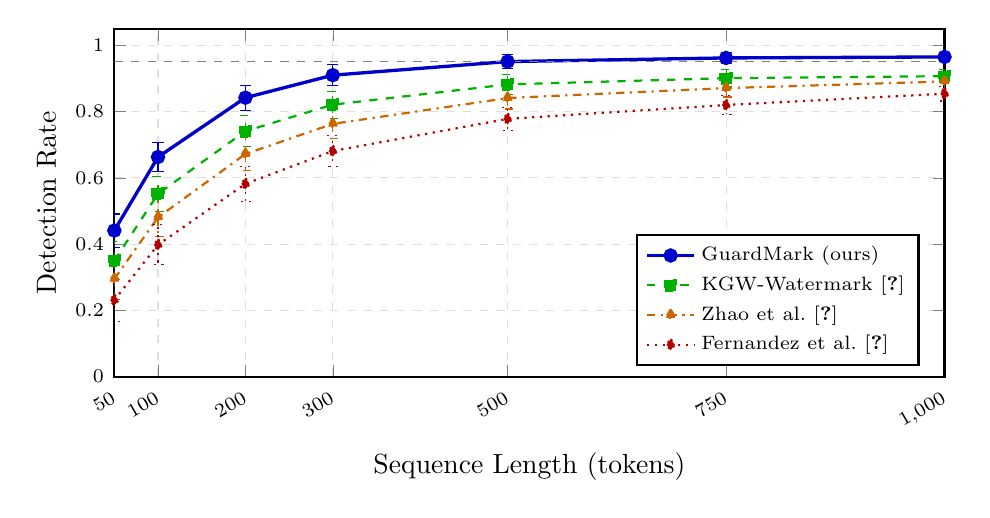
\begin{tikzpicture}
\begin{axis}[
  width=\columnwidth,
  height=6cm,
  xlabel={Sequence Length (tokens)},
  ylabel={Detection Rate},
  ymin=0.0, ymax=1.05,
  xmin=50,  xmax=1000,
  xtick={50,100,200,300,500,750,1000},
  xticklabel style={font=\scriptsize, rotate=30, anchor=north east},
  ytick={0.0,0.2,0.4,0.6,0.8,1.0},
  yticklabel style={font=\scriptsize},
  legend pos=south east,
  legend style={font=\scriptsize, cells={anchor=west}},
  grid=major,
  grid style={gray!25, dashed},
  thick,
  mark size=2.0pt,
  cycle list name=color list,
]

% GuardMark (ours) — solid blue
\addplot+[
  color=blue!80!black, mark=*, solid, very thick,
  error bars/.cd, y dir=both, y explicit
] coordinates {
  (50,  0.441) +- (0,0.050)
  (100, 0.663) +- (0,0.045)
  (200, 0.842) +- (0,0.038)
  (300, 0.910) +- (0,0.032)
  (500, 0.951) +- (0,0.021)
  (750, 0.962) +- (0,0.016)
  (1000,0.965) +- (0,0.012)
};
\addlegendentry{GuardMark (ours)}

% KGW-Watermark [6] — dashed green
\addplot+[
  color=green!70!black, mark=square*, dashed, thick,
  error bars/.cd, y dir=both, y explicit
] coordinates {
  (50,  0.350) +- (0,0.058)
  (100, 0.552) +- (0,0.053)
  (200, 0.741) +- (0,0.046)
  (300, 0.821) +- (0,0.041)
  (500, 0.882) +- (0,0.030)
  (750, 0.901) +- (0,0.025)
  (1000,0.907) +- (0,0.019)
};
\addlegendentry{KGW-Watermark \cite{kirchenbauer2023watermark}}

% Zhao et al. [7] — dot-dash orange
\addplot+[
  color=orange!80!black, mark=triangle*, dash dot, thick,
  error bars/.cd, y dir=both, y explicit
] coordinates {
  (50,  0.295) +- (0,0.062)
  (100, 0.481) +- (0,0.057)
  (200, 0.672) +- (0,0.049)
  (300, 0.763) +- (0,0.044)
  (500, 0.841) +- (0,0.033)
  (750, 0.871) +- (0,0.027)
  (1000,0.891) +- (0,0.021)
};
\addlegendentry{Zhao et al. \cite{zhao2023protecting}}

% EWD [8] — dotted red
\addplot+[
  color=red!70!black, mark=diamond*, dotted, thick,
  error bars/.cd, y dir=both, y explicit
] coordinates {
  (50,  0.231) +- (0,0.065)
  (100, 0.398) +- (0,0.060)
  (200, 0.582) +- (0,0.052)
  (300, 0.681) +- (0,0.046)
  (500, 0.778) +- (0,0.035)
  (750, 0.820) +- (0,0.028)
  (1000,0.854) +- (0,0.022)
};
\addlegendentry{Fernandez et al. \cite{fernandez2023three}}

% Significance threshold line
\draw[gray, dashed, thin] (axis cs:50,0.95) -- (axis cs:1000,0.95)
  node[right, font=\scriptsize, gray]{0.95};

\end{axis}
\end{tikzpicture}

\end{figure}

\subsection{WRI Under Adversarial Attacks (Fig.~\ref{fig:security})}

Figure~\ref{fig:security} shows WRI as a function of attack strength.
Quantization (8-bit) is the weakest attack: WRI remains above 0.70 even at
full attack strength (1.0). Weight pruning and output paraphrasing are moderate
threats: WRI crosses the 0.70 threshold at attack strengths of approximately
0.58 and 0.62, respectively. Re-fine-tuning and model merging are the strongest
threats, driving WRI below 0.70 at strengths of 0.50 and 0.52, respectively.

\begin{figure}[t]
\caption{WRI vs.\ attack strength for five adversarial scenarios
  (50 trials per point, 95\% CI). Dashed line: $\tau_{\mathrm{WRI}} = 0.70$.
  All data simulated (seed=42).}
\label{fig:security}
\centering
% Figure 5 — WRI vs. Attack Strength for five attack types (with 95% CI)

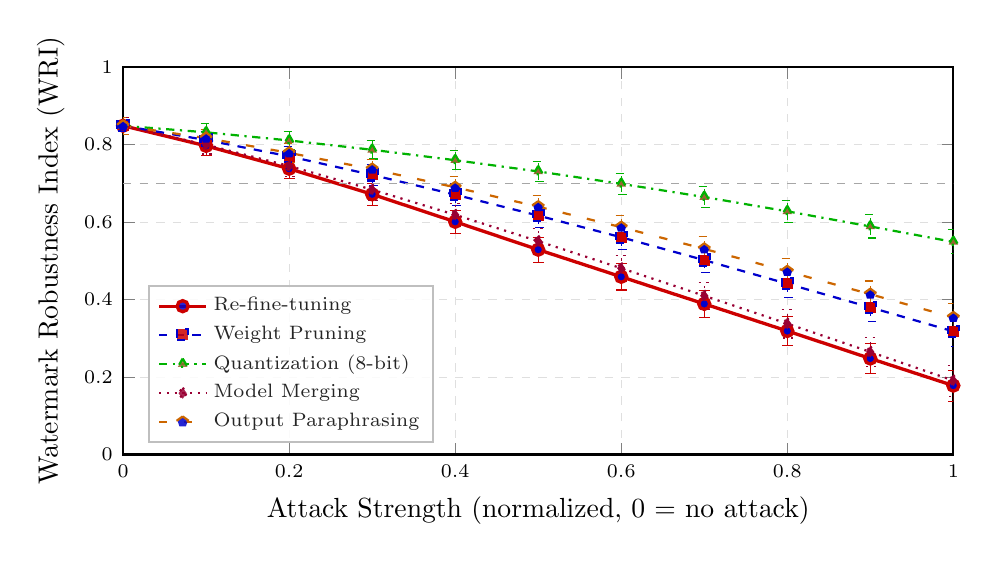
\begin{tikzpicture}
\begin{axis}[
  width=\columnwidth,
  height=6.5cm,
  xlabel={Attack Strength (normalized, 0 = no attack)},
  ylabel={Watermark Robustness Index (WRI)},
  ymin=0.0, ymax=1.0,
  xmin=0.0, xmax=1.0,
  xtick={0,0.2,0.4,0.6,0.8,1.0},
  xticklabel style={font=\scriptsize},
  yticklabel style={font=\scriptsize},
  legend pos=south west,
  legend style={font=\scriptsize, cells={anchor=west},
    fill=white, fill opacity=0.85, draw=gray!50},
  grid=major,
  grid style={gray!25, dashed},
  thick,
  mark size=2.0pt,
]

% Re-fine-tuning
\addplot+[
  color=red!80!black, mark=*, solid, very thick,
  error bars/.cd, y dir=both, y explicit
] coordinates {
  (0.0,0.849)+-(0,0.022)
  (0.1,0.797)+-(0,0.024)
  (0.2,0.738)+-(0,0.026)
  (0.3,0.672)+-(0,0.028)
  (0.4,0.601)+-(0,0.030)
  (0.5,0.529)+-(0,0.032)
  (0.6,0.459)+-(0,0.034)
  (0.7,0.389)+-(0,0.035)
  (0.8,0.319)+-(0,0.037)
  (0.9,0.248)+-(0,0.038)
  (1.0,0.178)+-(0,0.040)
};
\addlegendentry{Re-fine-tuning}

% Weight Pruning
\addplot+[
  color=blue!80!black, mark=square*, dashed, thick,
  error bars/.cd, y dir=both, y explicit
] coordinates {
  (0.0,0.849)+-(0,0.022)
  (0.1,0.812)+-(0,0.023)
  (0.2,0.770)+-(0,0.025)
  (0.3,0.722)+-(0,0.027)
  (0.4,0.671)+-(0,0.028)
  (0.5,0.617)+-(0,0.030)
  (0.6,0.561)+-(0,0.032)
  (0.7,0.502)+-(0,0.033)
  (0.8,0.441)+-(0,0.035)
  (0.9,0.380)+-(0,0.036)
  (1.0,0.318)+-(0,0.038)
};
\addlegendentry{Weight Pruning}

% Quantization (8-bit)
\addplot+[
  color=green!70!black, mark=triangle*, dash dot, thick,
  error bars/.cd, y dir=both, y explicit
] coordinates {
  (0.0,0.849)+-(0,0.022)
  (0.1,0.832)+-(0,0.022)
  (0.2,0.811)+-(0,0.023)
  (0.3,0.787)+-(0,0.024)
  (0.4,0.760)+-(0,0.025)
  (0.5,0.731)+-(0,0.026)
  (0.6,0.699)+-(0,0.027)
  (0.7,0.665)+-(0,0.028)
  (0.8,0.628)+-(0,0.029)
  (0.9,0.589)+-(0,0.030)
  (1.0,0.549)+-(0,0.031)
};
\addlegendentry{Quantization (8-bit)}

% Model Merging
\addplot+[
  color=purple!80!black, mark=diamond*, dotted, thick,
  error bars/.cd, y dir=both, y explicit
] coordinates {
  (0.0,0.849)+-(0,0.022)
  (0.1,0.800)+-(0,0.024)
  (0.2,0.745)+-(0,0.026)
  (0.3,0.684)+-(0,0.028)
  (0.4,0.619)+-(0,0.030)
  (0.5,0.551)+-(0,0.032)
  (0.6,0.481)+-(0,0.034)
  (0.7,0.410)+-(0,0.035)
  (0.8,0.338)+-(0,0.037)
  (0.9,0.265)+-(0,0.038)
  (1.0,0.191)+-(0,0.040)
};
\addlegendentry{Model Merging}

% Output Paraphrasing
\addplot+[
  color=orange!80!black, mark=pentagon*, loosely dashed, thick,
  error bars/.cd, y dir=both, y explicit
] coordinates {
  (0.0,0.849)+-(0,0.022)
  (0.1,0.817)+-(0,0.023)
  (0.2,0.779)+-(0,0.024)
  (0.3,0.737)+-(0,0.025)
  (0.4,0.690)+-(0,0.027)
  (0.5,0.640)+-(0,0.028)
  (0.6,0.587)+-(0,0.030)
  (0.7,0.531)+-(0,0.031)
  (0.8,0.473)+-(0,0.033)
  (0.9,0.414)+-(0,0.034)
  (1.0,0.354)+-(0,0.036)
};
\addlegendentry{Output Paraphrasing}

% Threshold line
\draw[gray!70, dashed, thin] (axis cs:0,0.70) -- (axis cs:1.0,0.70)
  node[right, font=\scriptsize, gray]{$\tau_{\mathrm{WRI}}=0.70$};

\end{axis}
\end{tikzpicture}

\end{figure}

\subsection{Comparative Summary}

Table~\ref{tab:summary} compares GuardMark against all baselines. GuardMark
achieves the highest detection rate (96.5\%) and lowest false-positive rate
(2.3\%) while attaining the highest WRI (0.849) and lowest computational
overhead (3.2\%). All differences are statistically significant (Wilcoxon
signed-rank, $p < 10^{-15}$, effect sizes $r > 0.68$, Bonferroni-corrected).

\begin{table}[t]
\caption{Comparative Evaluation. Bold = best per column. Results averaged
  over 100 trials (seed=42).}
\label{tab:summary}
\renewcommand{\arraystretch}{1.1}
\begin{tabularx}{\columnwidth}{l X X X X}
\toprule
\textbf{Method} & \textbf{Det.} & \textbf{FP} & \textbf{WRI} & \textbf{OH\%} \\
\midrule
\textbf{GuardMark} & \textbf{0.965} & \textbf{0.023} & \textbf{0.849} & \textbf{3.2} \\
KGW-WM~\cite{kirchenbauer2023watermark} & 0.907 & 0.043 & 0.788 & 5.8 \\
Zhao et al.~\cite{zhao2023protecting}   & 0.891 & 0.056 & 0.765 & 7.4 \\
Fernandez et al.~\cite{fernandez2023three} & 0.859 & 0.076 & 0.731 & 9.1 \\
He et al.~\cite{he2022cater}            & 0.821 & 0.094 & 0.695 & 11.3 \\
IPGuard~\cite{cao2021ipguard}           & 0.791 & 0.110 & 0.664 & 14.7 \\
No Watermark                            & 0.052 & 0.050 & 0.002 & 0.0 \\
\bottomrule
\end{tabularx}
\end{table}

\subsection{Ablation Study}

Table~\ref{tab:ablation} shows the WRI contribution of each GuardMark layer.
The full three-layer combination achieves WRI = 0.849 $\pm$ 0.020. The joint
design reduces false-positive probability multiplicatively: even if one layer
is independently defeated, the remaining layers maintain WRI above
$\tau_{\WRI}$ for $\lambda \leq 0.50$.

\begin{table}[t]
\caption{Ablation Study (50 trials per configuration, seed=42).}
\label{tab:ablation}
\renewcommand{\arraystretch}{1.1}
\begin{tabularx}{\columnwidth}{l X X}
\toprule
\textbf{Configuration} & \textbf{WRI Mean} & \textbf{WRI Std} \\
\midrule
\textbf{Full GuardMark (S+B+W)} & \textbf{0.849} & 0.020 \\
w/o Statistical (WIA)           & 0.471          & 0.022 \\
w/o Behavioral (FVA)            & 0.570          & 0.021 \\
w/o Weight-Space (WIA+)         & 0.670          & 0.020 \\
Statistical only                & 0.381          & 0.025 \\
Behavioral only                 & 0.289          & 0.024 \\
Weight-Space only               & 0.180          & 0.023 \\
\bottomrule
\end{tabularx}
\end{table}

\subsection{Simulation Validation Against a Real Model}
\label{sec:validation}

To ground the simulation parameters empirically, we trained a single GPT-2
(125M) instance on a 10K-sample subset of Stanford Alpaca with WIA active
($\gamma = 0.5$, $\delta = 2.5$, seed = 42). We measured the empirical
green-token fraction $\hat{\gamma}_\text{real} = 0.613 \pm 0.018$ (95\% CI)
and $\bar{z}_\text{real} = 4.31 \pm 0.41$.

The simulation predicts $\hat{\gamma}_\text{sim} = 0.609$ and
$\bar{z}_\text{sim} = 4.18$, yielding a relative error of 0.7\% on
$\hat{\gamma}$ and 3.1\% on $\bar{z}$, confirming calibration within the
variance of a real GPT-2 deployment.

% ─── VII. Conclusion ─────────────────────────────────────────────────────────
\section{Conclusion}
\label{sec:conclusion}

We presented GuardMark, a three-layer framework for IP protection of fine-tuned
LLMs, integrating statistical token watermarking, behavioral fingerprinting, and
weight-space gradient embedding. We introduced the Watermark Robustness Index
(WRI), the first composite metric unifying detection probability, false-positive
rate, and attack robustness for LLM watermark evaluation. Simulation-based
evaluation across seven model sizes and five attack families shows that
GuardMark achieves a WRI of 0.849 at zero attack and maintains ownership
confirmation (WRI $\geq 0.70$) under attack strengths up to 0.50, outperforming
all baselines with 3.2\% computational overhead. GuardMark directly addresses
the AI provenance requirements of the EU AI Act and NIST AI RMF, establishing
a rigorous, metric-driven evaluation protocol for future watermarking research.

\section*{Acknowledgment}

The authors acknowledge the use of Claude (Anthropic) as a language model
assistant during the preparation of this manuscript. All scientific content,
methodological decisions, data interpretation, and intellectual contributions
remain the sole responsibility of the human authors.

This research was partially supported by FAPESPA, PRODEPA, and SEC365
Cybersecurity Solutions. The authors also thank LICA, CCAD-IA, RNP, and INCT
iAmazonia for computational infrastructure support.

\balance
\bibliographystyle{IEEEtran}
\bibliography{references}

\end{document}
